\documentclass[a4paper,12pt,headsepline]{scrartcl}

%\part{title}
\usepackage[utf8]{inputenc}
\usepackage{graphicx}
\usepackage{caption,subcaption}
\usepackage[british]{babel}
\usepackage[T1]{fontenc}
\usepackage{geometry}
\usepackage{proof}
\geometry{left=3.5cm, right=2cm, top=2.5cm, bottom=2cm}
\usepackage{hyperref}
%\usepackage[hyphens,obeyspaces,spaces]{url}
\usepackage{fancybox}
\usepackage{amssymb,amsmath,amsthm}
\usepackage{gensymb}
\usepackage[linesnumbered,ruled,vlined,norelsize]{algorithm2e}
%\usepackage[bookmarksnumbered,pdftitle={\titleDocument},hyperfootnotes=false]{hyperref} 
\usepackage{color}
\usepackage{float}
\usepackage{enumerate}
\usepackage{marvosym}
\usepackage{tikz}
\usetikzlibrary{positioning}
\usetikzlibrary{patterns}
\usepackage{pgfplots}
\pgfplotsset{compat=1.12}
\usepgfplotslibrary{fillbetween}
%%%

% Always forgetting the figure parameters for precise graphical inclusions -.-

%\begin{figure}[H]
	%\centering
	%\begin{subfigure}{0.4\textwidth}
		%\centering
		%\includegraphics[width=0.34\linewidth,page=6]{includegraphics/L-%t-shape_candidates}
%		\caption{Empty $T$-face}\label{im:empty_T}	
%	\end{subfigure}
%%%
%test
%\usepackage[backend=bibtex]{biblatex}
%\usepackage{filecontents}

%\addbibresource{ref.bib}

\restylefloat{figure}

% Makros
%\newenvironment{sketch}{\begin{proof}[Proof (Sketch)]}{\end{proof}}
%\newtheorem{theorem}{Theorem}
%\newtheorem{assumption}{Assumption}
\newtheorem{lemma}{Lemma}
%\newtheorem{remark}{Remark}
%\newtheorem{definition}{Definition}
%\newtheorem{corollary}{Corollary}
\newcommand{\comment}[1]
{
  \begin{quotation}
    \textcolor{blue}{\underline{Edit:} #1}
  \end{quotation}
}
\newtheorem{aufgabe}{Exercise}
\newcommand{\Ex}[2]
{
	\setcounter{section}{#2}
	\section*{Übungsblatt #2 zu #1}
}
\newcommand{\TODO}[1]
{
  \begin{quotation}
    \textcolor{red}{\underline{TODO:} #1}
  \end{quotation}
}
% Zeichen 
\newcommand{\OO}{\ensuremath{\mathcal{O}}}
\newcommand{\ec}{\texttt{ec}}
\newcommand{\NP}{\call{NP}}
\newcommand{\call}[1]{\ensuremath{\mathcal{#1}}}

% neue Kopfzeilen mit fancypaket
\usepackage{fancyhdr} %Paket laden
\pagestyle{fancy} %eigener Seitenstil
\fancyhf{} %alle Kopf- und Fußzeilenfelder bereinigen
\fancyhead[L]{Benjamin \c Coban \\ Christoph Jabs}
\fancyhead[C]{Algorithmen und Komplexität \\ Blatt 7}
\fancyhead[R]{3526251 \\ 5567177}
\setlength{\headheight}{39pt}
\renewcommand{\headrulewidth}{0.4pt} %obere Trennlinie
%\fancyfoot[C]{\thepage} %Seitennummer
%\renewcommand{\footrulewidth}{0.4pt} %untere Trennlinie

\frenchspacing
\makeindex

% Pseudocode für Java
\usepackage{listings}
\lstset{numbers=left, numberstyle=\tiny, numbersep=5pt, keywordstyle=\color{black}\bfseries, stringstyle=\ttfamily,showstringspaces=false,basicstyle=\footnotesize,captionpos=b}
\lstset{language=java}

% Disable single lines at the start of a paragraph (Schusterjungen)
\clubpenalty = 10000
% Disable single lines at the end of a paragraph (Hurenkinder)

\widowpenalty = 10000
\displaywidowpenalty = 10000
\begin{document}
\begin{aufgabe}
\end{aufgabe}
As a first step for solving the Linear Program, we define the dual LP:
\begin{alignat*}{4}
  & \textbf{min}\quad  & \beta y_0 +\sum_{j=1}^n y_j \\
  & \textbf{s.t.}\quad & y_0q_j    + y_j             & \ge p_j & \quad\forall j=1,\dots,n \\
  &                    & y_j                         & \ge 0   & \quad\forall j=1,\dots,n
\end{alignat*}

As a next step, we modify the dual problem, so that it is in standard form and we divide the constraints by $q_j$.
\begin{alignat*}{4}
  & \textbf{max}\quad  & -\beta y_0 -\sum_{j=1}^n y_j \\
  & \textbf{s.t.}\quad & -y_0       - \frac{y_j}{q_j} & \le -\frac{p_j}{q_j} & \quad\forall j=1,\dots,n \\
  &                    & y_j                          & \ge 0                & \quad\forall j=1,\dots,n
\end{alignat*}

Now we can formulate this LP in slack form as a dictionary.
\begin{alignat*}{2}
  z       &= -\beta y_0 -\sum_{j=1}^n y_j \\
  y_{n+j} &= -\frac{p_j}{q_j} + y_0 + \frac{y_j}{q_j} & \quad\forall j=1,\dots,n
\end{alignat*}

Since the initial solution of the simplex method for this LP is not feasible, we look at the auxiliary LP:
\begin{alignat*}{2}
  z       &= -y_\text{aux} \\
  y_{n+j} &= -\frac{p_j}{q_j} + y_0 + \frac{y_j}{q_j} + y_\text{aux} & \quad\forall j=1,\dots,n
\end{alignat*}

We choose $y_\text{aux}$ as the entering variable.
Since $-\frac{p_n}{q_n}$ is the ``most infeasible'', we choose $y_{2n}$ as the leaving variable.
\[ \Rightarrow\quad y_\text{aux} = y_{2n}+\frac{p_n}{q_n}-y_0-\frac{y_n}{q_n} \]
\begin{alignat*}{2}
  z            &= -\frac{p_n}{q_n}+y_0+\frac{y_n}{q_n}-y_{2n} \\
  y_{n+j}      &= \frac{p_n}{q_n}-\frac{p_j}{q_j}-\frac{y_n}{q_n}+\frac{y_j}{q_j}+y_{2n} & \quad\forall j=1,\dots,n-1 \\
  y_\text{aux} &= \frac{p_n}{q_n}-y_0-\frac{y_n}{q_n}+y_{2n}
\end{alignat*}

Because $\sum_{j=1}^n q_j=1$ and $q_j>0\,\forall j=1,\dots,n$, we know that $q_j\le1\,\forall j=1,\dots,n$.
Therefore $y_n$ is chosen as the entering variable, because $\frac{1}{q_n}\ge1$.
Since $y_n$ has the same coefficient in all constraints, we choose the constraint with the smallest constant as the leaving variable.
This is $y_{2n-1}$.
\[ \Rightarrow\quad y_n = q_n\left(\frac{p_n}{q_n}-\frac{p_{n-1}}{q_{n-1}}+\frac{y_{n-1}}{q_{n-1}}-y_{2n-1}+y_{2n}\right) \]
\begin{alignat*}{2}
  z            &= -\frac{p_{n-1}}{q_{n-1}}+y_0+\frac{y_{n-1}}{q_{n-1}}-y_{2n-1} \\
  y_{n+j}      &= \frac{p_{n-1}}{q_{n-1}}-\frac{p_j}{q_j}-\frac{y_{n-1}}{q_{n-1}}+\frac{y_j}{q_j}+y_{2n-1} & \quad\forall j=1,\dots,n-2 \\
  y_\text{aux} &= \frac{p_{n-1}}{q_{n-1}}-y_0-\frac{y_{n-1}}{q_{n-1}}+y_{2n-1} \\
  y_n          &= q_n\left(\frac{p_n}{q_n}-\frac{p_{n-1}}{q_{n-1}}+\frac{y_{n-1}}{q_{n-1}}-y_{2n-1}+y_{2n}\right)
\end{alignat*}

This step is repeated for $i=1,\dots,n-1$ times where always $y_{n-i+1}$ is chosen as the entering and $y_{2n-i}$ as the leaving variable.
After step $i$ we therefore have the following dictionary:
\begin{alignat*}{2}
  z            &= -\frac{p_{n-i}}{q_{n-i}}+y_0+\frac{y_{n-i}}{q_{n-i}}-y_{2n-i} \\
  y_{n+j}      &= \frac{p_{n-i}}{q_{n-i}}-\frac{p_j}{q_j}-\frac{y_{n-i}}{q_{n-i}}+\frac{y_j}{q_j}+y_{2n-i} & \quad\forall j=1,\dots,n-i-1 \\
  y_\text{aux} &= \frac{p_{n-i}}{q_{n-i}}-y_0-\frac{y_{n-i}}{q_{n-i}}+y_{2n-i} \\
  y_{n-j}      &= q_{n-j}\left(\frac{p_{n-j}}{q_{n-j}}-\frac{p_{n-i}}{q_{n-i}}+\frac{y_{n-i}}{q_{n-i}}-y_{2n-i}+y_{2n-j}\right) & \quad\forall j=0,\dots,i-1
\end{alignat*}

After the last step ($i=n-1$), we therefore get the following dictionary:
\begin{alignat*}{2}
  z            &= -\frac{p_{1}}{q_{1}}+y_0+\frac{y_{1}}{q_{1}}-y_{n+1} \\
  y_\text{aux} &= \frac{p_{1}}{q_{1}}-y_0-\frac{y_{1}}{q_{1}}+y_{n+1} \\
  y_{n-j}      &= q_{n-j}\left(\frac{p_{n-j}}{q_{n-j}}-\frac{p_{1}}{q_{1}}+\frac{y_{1}}{q_{1}}-y_{n+1}+y_{2n-j}\right) & \quad\forall j=0,\dots,n-2
\end{alignat*}

Now we can do one final step where $y_1$ is the entering and $y_\text{aux}$ is the leaving variable:
\[ \Rightarrow\quad y_1 = q_1\left(\frac{p_1}{q_1}-y_0+y_{n+1}-y_\text{aux}\right) \]
\begin{alignat*}{2}
  z            &= -y_\text{aux} \\
  y_j      &= q_j\left(\frac{p_j}{q_j}-y_0-y_\text{aux}+y_{n+j}\right) & \quad\forall j=1,\dots,n
\end{alignat*}

This tells us our initial solution for the modified dual LP:
\[ \hat{y}_j = \begin{cases}0&\text{for}\,j=0\\ p_j&\text{for}\,j=1,\dots,n\\0&\text{for}\,j=n+1,\dots,2n\end{cases} \]

Now we go back to the modified dual problem by dropping $y_\text{aux}$ and changing the objective function.
\[ z = -\beta y_0-\sum_{j=1}^n y_j = -\beta y_0 -\sum_{j=1}^n p_j +\sum_{j=1}^n q_jy_0 -\sum_{j=1}^n q_jy_{n+j} = (1-\beta)y_0-1-\sum_{j=1}^n q_jy_{n+j} \]
\begin{alignat*}{2}
  z   &= -1+(1-\beta)y_0-\sum_{j=1}^n q_jy_{n+j} \\
  y_j &= q_j\left(\frac{p_j}{q_j}-y_0+y_{n+j}\right) & \quad\forall j=1,\dots,n
\end{alignat*}

From $\frac{\beta}{q_j}<1\,\forall j=1,\dots,n$, we know that $\beta<q_j\,\forall j=1,\dots,n$ and therefore $1-\beta>0$.
Therefore we choose $y_0$ as the entering variable.
From each of the constraints, we find that we can increase $y_0$ to a maximum of $\frac{p_j}{q_j}$.
This is smallest for the constraint for $y_1$, which is therefore chosen as the leaving variable.
\[ y_0 = \frac{p_1}{q_1}-\frac{y_1}{q_1}+y_{n+1} \]
\begin{alignat*}{2}
  z   &= (1-\beta)\frac{p_1}{q_1}-1-(1-\beta)\frac{y_1}{q_1}+(1-\beta-q_1)y_{n+1}-\sum_{j=2}^n q_jy_{n+j} \\
	y_j &= q_j\left(\frac{p_j}{q_j}-\frac{p_1}{q_1}+\frac{y_1}{q_1}+y_{n+j}-y_{n+1}\right) & \quad\forall j=2,\dots,n \\
	y_0 &= \frac{p_1}{q_1}-\frac{y_1}{q_1}+y_{n+1}
\end{alignat*}

We know that $\sum_{j=1}^n q_j = 1$ and that $\beta<q_j\,\forall j=1\dots,n$, therefore we know that a sum over not all $q_j$ is smaller then $1-\beta$.
Because of this, we know that $1-\beta-q_1>0$ and we choose $y_{n+1}$ as the leaving variable.
For each constraint we can increase $y_{n+1}$ to a maximum of $\frac{p_j}{q_j}$, we therefore choose $y_2$ as the leaving variable.
\[ y_{n+1} = \frac{p_2}{q_2}-\frac{p_1}{q_1}+\frac{y_1}{q_1}-\frac{y_2}{q_2}+y_{n+2} \]
\begin{alignat*}{2}
  z       &= -1 + p_1 - y_1 + (1-\beta-q_1)(\frac{p_2}{q_2} - \frac{y_2}{q_2}) + (1-\beta-q_1-q_2)y_{n+2} - \sum_{j=3}^n q_jy_{n+j} \\
	y_j     &= q_j\left(\frac{p_j}{q_j}-\frac{p_2}{q_2}+\frac{y_2}{q_2}+y_{n+j}-y_{n+2}\right) \quad\forall j=3,\dots,n \\
	y_0     &= \frac{p_2}{q_2}-\frac{y_2}{q_2}+y_{n+2} \\
	y_{n+1} &= \frac{p_2}{q_2}-\frac{p_1}{q_1}+\frac{y_1}{q_1}-\frac{y_2}{q_2}+y_{n+2}
\end{alignat*}

This step does now again repeat for $i=2,\dots,n$ and we can formulate the dictionary after the $i$th step as follows:
\begin{alignat*}{2}
  z       &= -1 + \sum_{j=1}^{i-1} \left(p_j - y_j\right) + (1-\beta-\sum_{j=1}^{i-1} q_j)(\frac{p_i}{q_i} - \frac{y_i}{q_i}) + (1-\beta-\sum_{j=1}^i q_j)y_{n+i} - \sum_{j=i+1}^n q_jy_{n+j} \\
	y_j     &= q_j\left(\frac{p_j}{q_j}-\frac{p_i}{q_i}+\frac{y_i}{q_i}+y_{n+j}-y_{n+i}\right) \quad\forall j=i+1,\dots,n \\
	y_0     &= \frac{p_i}{q_i}-\frac{y_i}{q_i}+y_{n+i} \\
	y_{n+j} &= \frac{p_i}{q_i}-\frac{p_j}{q_j}+\frac{y_j}{q_j}-\frac{y_i}{q_i}+y_{n+i} \quad\forall j=1,\dots,i-1
\end{alignat*}

After the last step ($i=n$), we therefore get the following dictionary:
\begin{alignat*}{2}
  z       &= -1 + \sum_{j=1}^{n-1} \left(p_j - y_j\right) + (1-\beta-\sum_{j=1}^{n-1} q_j)(\frac{p_n}{q_n} - \frac{y_n}{q_n}) -\beta y_{2n} \\
	y_0     &= \frac{p_n}{q_n}-\frac{y_n}{q_n}+y_{2n} \\
	y_{n+j} &= \frac{p_n}{q_n}-\frac{p_j}{q_j}+\frac{y_j}{q_j}-\frac{y_n}{q_n}+y_{2n} \quad\forall j=1,\dots,n-1
\end{alignat*}

Here, all coefficients in the objective function are negative and the simplex method does therefore terminate.
We get the following optimal solution for the (modified) dual problem:
\[ y^*_j = \begin{cases}\frac{p_n}{q_n}&\text{for}\,j=0\\0&\forall j=1,\dots,n\\\frac{p_n}{q_n}-\frac{p_{n-j}}{q_{n-j}}&\forall j=n,\dots,2n-1\\0&\text{for}\,j=2n\end{cases} \]

We can now find the solution for the primal problem with the help of the complementary slackness theorem.
We know that where the dual solution is $\neq 0$, the primal constraint needs to be tight, therefore since $y_0\neq 0$ we know that
\begin{equation}\label{eq:tight}
	\sum_{j=1}^n q_jx_j=\beta
\end{equation}
In addition to that, we know that where the constraints of the dual are slack, the primal value needs to be zero.
In the constraints of the dual we see the following:
\begin{alignat*}{2}
	-y_0+\frac{y_j}{q_j} &\le -\frac{p_j}{q_j} & \forall j=1,\dots,n \\
	\Rightarrow\quad -y_0 &\le -\frac{p_j}{q_j} & \forall j=1,\dots,n \\
	\Rightarrow\quad -\frac{p_n}{q_n} &\le -\frac{p_j}{q_j} & \forall j=1,\dots,n
\end{alignat*}
We can see that all constraints are slack, except for the one for $j=n$.
Therefore we know that $x_j = 0\,\forall j=1,\dots,n-1$.

From that and \eqref{eq:tight}, we can now compute $x_n$:
\[ \sum_{j=1}^n q_jx_j = \beta = q_nx_n \quad\Rightarrow\quad x_n=\frac{\beta}{q_n} \]

The final (optimal) solution to the primal problem is therefore:
\[ x^*_j = \begin{cases}0&\forall j=1,\dots,n\\\frac{\beta}{q_n}&\text{for}\,j=n\end{cases} \]

\newpage
\begin{aufgabe}
\end{aufgabe}
The Manhattan metrics between two points out of $\mathbb{R}^2$ is defined as:
\begin{align*}
d(p_i,p_j) = |x_i - x_j| + |y_i - y_j|
\end{align*}
\begin{enumerate}[a)]
	\item In the following figure, the rectangles along with the points of minimum distances are illustrated:
	\begin{figure}[H]
		\centering
		\begin{subfigure}{0.48\textwidth}
			\centering
			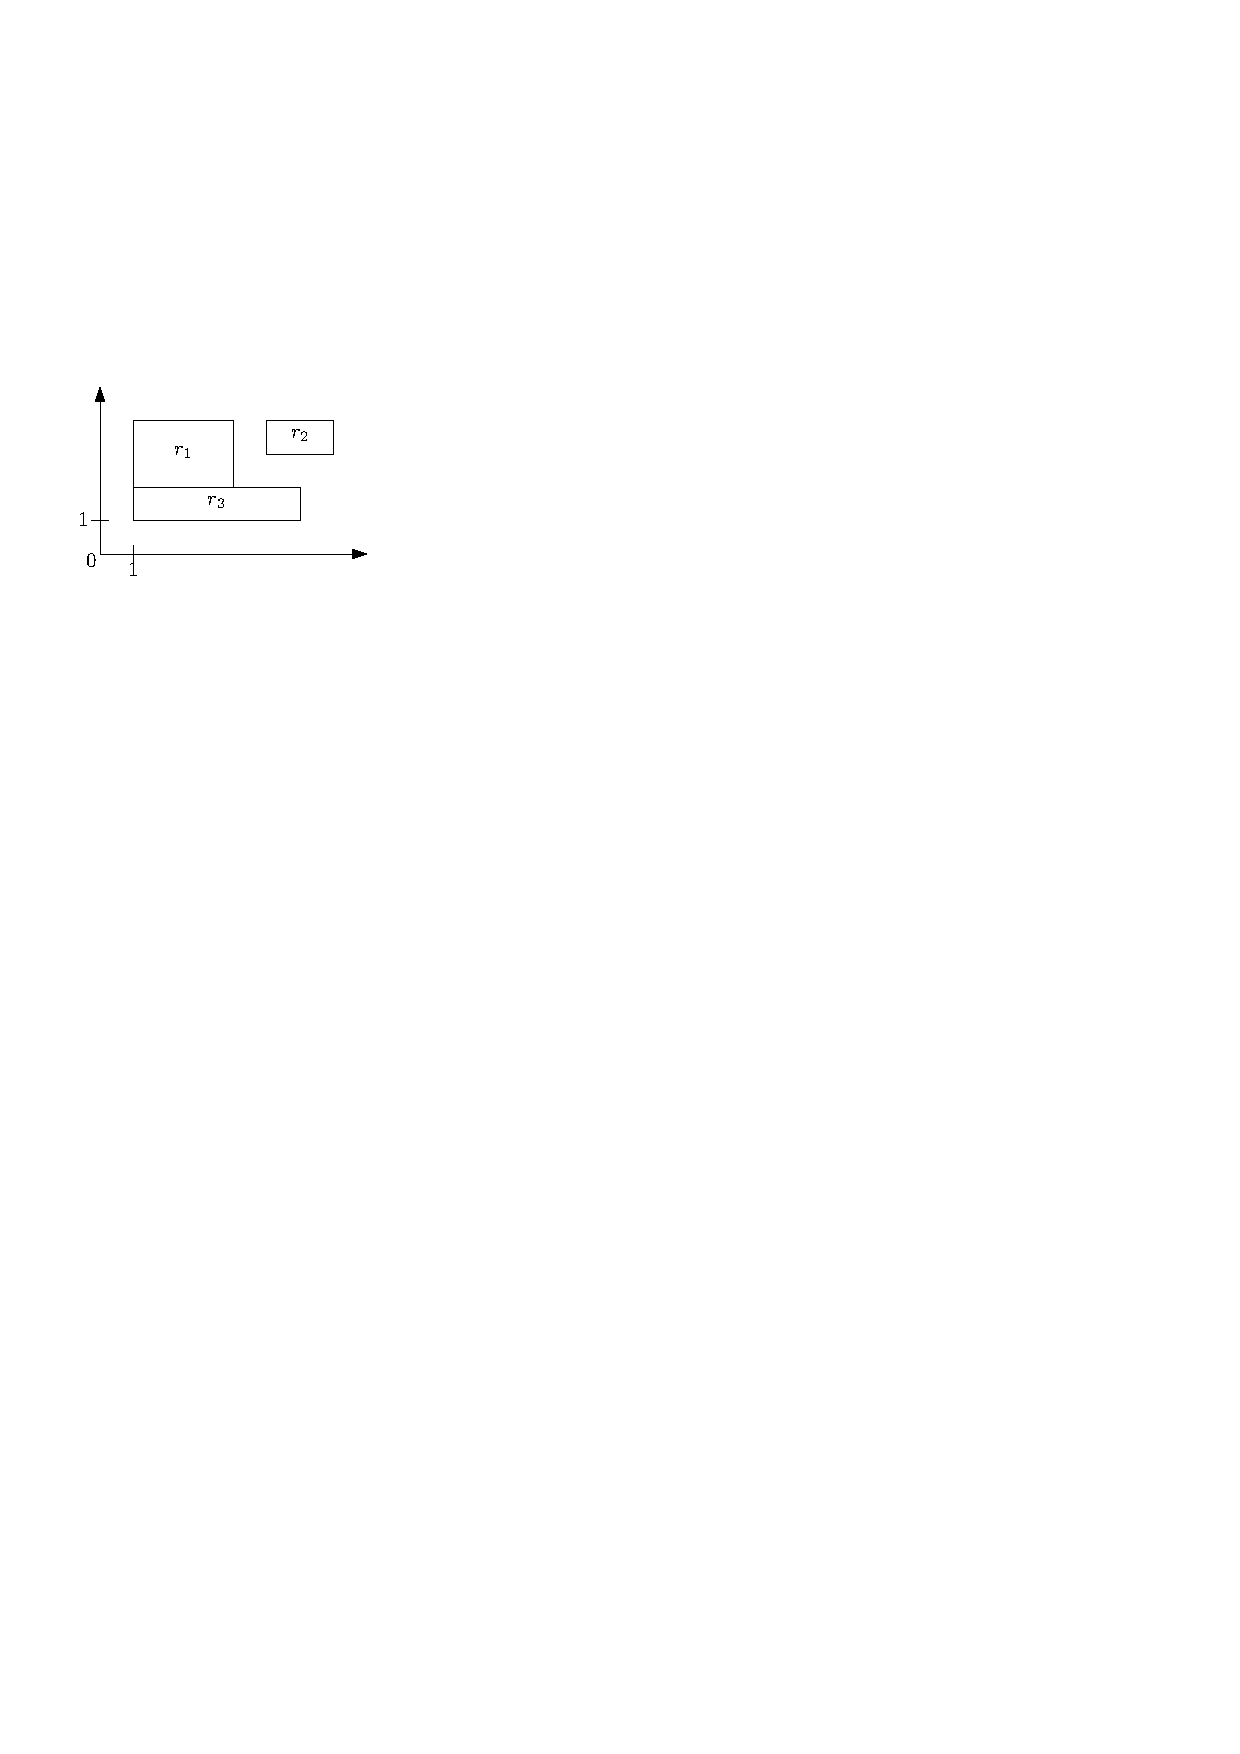
\includegraphics[width=1\linewidth,page=1]{graphics/7_2.pdf}
			\caption*{Illustration of the given rectangles}
		\end{subfigure}
		\begin{subfigure}{0.48\textwidth}
			\centering
			\includegraphics[width=1\linewidth,page=2]{graphics/7_2.pdf}
			\caption*{Solution to the given MMDPS problem}
		\end{subfigure}
	\end{figure}
An optimal solution is:
\begin{align*}
	p_1 = (4,2.5), p_2 = (5,3), p_3 = (5,2)
\end{align*}
with a diameter of 1.5.
\begin{proof}
	The minimum distance from $r_2$ to $r_1$ or $r_3$ is 1 due to the gap. To keep the distance to $r_3$ in $y$ direction and to $r_1$ in $x$ direction minimal, $p_2$ is set to the bottom left corner. Then, with two distances of 1, there is a diameter of 2 since the point set would span a square at its corners. So, the lower bound of the diameter is 1, the upper bound 2 with this approach.\\
	Next, it is to show that there is no point set with a lower diameter of 1.5. Suppose, there exists a point set $p'_1,p'_2, p'_3$ with fixed $p'_2 = p_2$ and a diameter of less than 1.5. Then, $d(p'_i,p_j') < 1.5$. Look at w.l.o.g. fixed $p'_2, p'_1$. Then, every point $p'_3$ fulfilling the diameter constraint is not in $r_3$, for all fixed points, contradicting the Minimum Manhattan Diameter Point Set.
\end{proof}
Note that this is not the only optimal solution, consider this second solution in the figure below:
	\begin{figure}[H]
	\centering
	\begin{subfigure}{0.48\textwidth}
		\centering
		\includegraphics[width=1\linewidth,page=3]{graphics/7_2.pdf}
		\caption*{Alternative solution}
	\end{subfigure}
\end{figure}
\item The following LP formulates the MMDPS. 
\begin{align*}
	\textbf{\text{min}} & z && && & &
\end{align*}
\begin{align}
	\textbf{\text{s.t.}} & &&x_i - &&x_l^i&&&& &\geq 0&\\
	                     & &&x_r^i - &&x_i&&&& &\geq 0&\\
	                     & &&y_t^i - &&y_i&&&& &\geq 0&\\
	                     & &&y_i - && y_b^i &&&& &\geq 0 &\\
	                     & && x_i - &&x_j + &&y_i - &&y_j &\leq z&\\
	                     & & -&x_i + &&x_j + &&y_i - &&y_j &\leq z&\\
	                     & && x_i - &&x_j + &-&y_i + &&y_j &\leq z&\\
	                     & & -&x_i + &&x_j + &-&y_i + &&y_j &\leq z&\\
	                     &&&&&&&&&&&\forall i,j\in \{1,...,n\}, i\neq j
\end{align}
Constraints 1 to 4 state that the points shall be in the rectangles. Constraints 5 to 8 formulate the Manhattan distance by resolving a non-linear inequality with two linear inequalitites. $z$ will be the diameter to minimize.
\end{enumerate}

\newpage
\begin{aufgabe}
\end{aufgabe}
In order to solve the given LP with the primal-dual method, we first formulate the dual problem $(D)$:
\begin{alignat*}{2}
	(D) \\
	\textbf{max}\quad  && 2y_1 + y_2 \\
	\textbf{s.t.}\quad && y_1 - y_2 &\le 2 \\
								     && -2y_1 + 3y_2 &\le 1
\end{alignat*}

As the initial solution for $(D)$, we use $y^{(0)}=(0,0)^T$ and based on that formulate the first iteration of the set $I$:
\[ I\left(y^{(0)}\right) = \left\{ j\,|\,1\le j\le 2 \vee \sum_i a_{ij}y^{(0)}_i=c_j \right\} = \emptyset \]

Based on that we can formulate the first restricted problem:
\begin{alignat*}{2}
	(R^{(0)}) \\
	\textbf{min}\quad  && s_1 + s_2 \\
	\textbf{s.t.}\quad && s_1 &= 2 \\
								     && s_2 &= 1 \\
								     && s &\ge 0
\end{alignat*}
The solution for that is obviously $s^{*(0)} = (2,1)^T$.

Now we consider the dual of this problem:
\begin{alignat*}{2}
	(DR^{(0)}) \\
	\textbf{max}\quad  && 2\pi_1 + \pi_2 \\
	\textbf{s.t.}\quad && \pi &\le 1
\end{alignat*}
which has the solution $\pi^{*(0)} = (1,1)^T$.

Now we want to improve the solution to the dual problem.
For that consider all $j\in\bar{I}$ and find that for $j=2$, $\sum_i a_{ij}\pi_i^{*(0)} > 0$.
Therefore we get the following $t$:
\[ t^{(0)} = \min_{j\in\bar{I}} \frac{c_j-\sum_i a_{ij}y_i^{(0)}}{\sum_i a_{ij}\pi_i^{*(0)}} = \frac{c_2-\sum_i a_{i2}y_i^{(0)}}{\sum_i a_{i2}\pi_i^{*(0)}} = 1 \]

Now we improve $y$
\[ y^{(1)} = y^{(0)} + t^{(0)}\pi^{*(0)} = (1,1)^T \]
and get a new set $I$:
\[ I\left(y^{(1)}\right) = \{2\} \]

We formulate the restricted problem:
\begin{alignat*}{2}
	(R^{(1)}) \\
	\textbf{min}\quad  && s_1 + s_2 \\
	\textbf{s.t.}\quad && -2x_2 + s_1 &= 2 \\
										 && 3x_2 + s_2 &= 1 \\
										 && x_2 &\ge 0 \\
								     && s &\ge 0
\end{alignat*}
and find the solution with the help of an LP solver\footnote{\url{https://online-optimizer.appspot.com}}: $s^{*(1)} = (\frac{2}{3},0)^T$.

We formulate the dual restricted problem:
\begin{alignat*}{2}
	(DR^{(1)}) \\
	\textbf{max}\quad  && 2\pi_1 + \pi_2 \\
	\textbf{s.t.}\quad && -2\pi_1 + 3\pi_2 &\le 0 \\
										 && \pi &\le 1
\end{alignat*}
which has the solution $\pi^{*(1)} = (1,\frac{2}{3})^T$.

We look at all $j\in\bar{I}$ and find that for $j=2$, $\sum_i a_{ij}\pi_i^{*(0)} > 0$.
Therefore we get the following $t$:
\[ t^{(1)} = \frac{c_1-\sum_i a_{i1}y_i^{(0)}}{\sum_i a_{i1}\pi_i^{*(0)}} = 6 \]

We improve $y$ again:
\[ y^{(2)} = y^{(1)} + t^{(1)}\pi^{*(1)} = (7,5)^T \]
and get a new set $I$:
\[ I\left(y^{(2)}\right) = \{1,2\} \]

We formulate the restricted problem:
\begin{alignat*}{2}
	(R^{(2)}) \\
	\textbf{min}\quad  && s_1 + s_2 \\
	\textbf{s.t.}\quad && x_1 + -2x_2 + s_1 &= 2 \\
										 && -x_1 + 3x_2 + s_2 &= 1 \\
										 && x &\ge 0 \\
								     && s &\ge 0
\end{alignat*}
and find the solution $s^{*(2)} = (0,0)^T$.
Since the objective function of the restricted problem is 0, we know that $y^{(2)}$ is optimal for $(D)$ and that $x^* = (8,3)^T$ as given by the solution of the restricted problem is the optimal solution for the primal problem.

\end{document}
